
%%%%%%%%%%%%%%%%%%%%%%%%%%%%%%%%  ejemplo.tex %%%%%%%%%%%%%%%%%%%%%%%%%%%%%%%

%%%%% Fichero de ejemplo LaTeX que ilustra el uso de la Hoja de Estilo %%%%%%
%%%%% Jornadas.cls para las XXII Jornadas de Paralelismo.              %%%%%%

\documentclass[twocolumn,twoside]{Jornadas}
\usepackage{fontspec}
\usepackage{xunicode}
\usepackage{xltxtra}
\usepackage{graphicx}
\graphicspath{{imgs/}}

\usepackage{listings}
\usepackage{color}
\lstloadlanguages{Python}
\lstset{
  language=Python,                      % C,Fortran,XML
  basicstyle=\scriptsize,               % Listados en small
  keywordstyle=\color{red},             % Palabras clave en rojo
  identifierstyle=\ttfamily,
  escapeinside={(*@}{@*)},
  commentstyle=\color{blue},            % comentarios en azul
  stringstyle=\color{green},            % cadenas en verde
  showstringspaces=false,
  frame=tb,
  captionpos=t,
  belowcaptionskip=12pt,
  stepnumber=2,                                         % Opciones de lineas y etiquetas
  numberstyle=\scriptsize,
  numbersep=5pt,
  tabsize=1
}


%%%%%%%%%%%%%%%%%%%%%%%%%%%%%%%%%%%%%%%%%%%%

\begin{document}


\title{Experiencias con Python y CUDA en Computación de Altas Prestaciones}

\author{Sergio Armas,%
     Lionel Mena,%
     Alejandro Samarín,% 
     Vicente Blanco%
     \thanks{Dpto. Estadística, I.O. y Computación, Univ. La Laguna, e-mail: {\tt vblanco@ull.es}},%
     Alberto Morales y % 
     Francisco Almeida
}

\maketitle
% Oculta las cabeceras y los números de página.
% Ambos elemetos se añadirán durante la edición de las actas completas.
\markboth{}{}
\pagestyle{empty} 
\thispagestyle{empty} % Oculta el número de la primera página

\begin{abstract}
La computacion...
\end{abstract}

\begin{keywords}
Python, CUDA, PyCUDA
\end{keywords}

\section{Introducción}

PyCUDA es un wrapper de Python para CUDA desarrollado por Andreas Kl\"{o}ckner. En este art\'{i}culo se har\'{a} un estudio acerca de si las ventajas de utilizar un lenguaje interpretado de muy alto nivel para ejecutar algoritmos en una GPU compensa la menor velocidad inherente a los lenguajes de script.
Para ello, se abordan dos problemas caracter\'{i}sticos: el producto matricial y la detecci\'{o}n de movimiento.

\ldots utilizando PyCUDA~\cite{DBLP:journals/corr/abs-0911-3456}

y una gráfica \ref{fig:Fermi}

\begin{figure}
	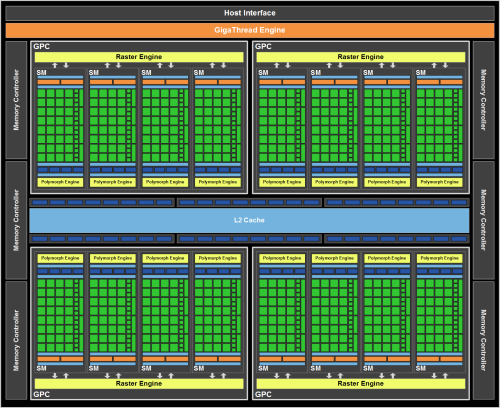
\includegraphics[width=.45\textwidth]{block_diagram_Fermi}
	\caption{\label{fig:Fermi} Diagrama de bloques de una GPU Tesla M2070 (Fermi)}
\end{figure}

y un código \ref{code:filter}


\section{Producto matricial}

La manera tradicional de abordar la multiplicaci\'{o}n de matrices pasa por ejecutar un algoritmo secuencial de complejidad casi c\'{u}bica en las mejores implementaciones. Su versi\'{o}n paralela, en cambio, permite el c\'{a}lculo simult\'{a}neo de las filas de la primera matriz multiplicando con la correspondiente columna de la segunda para formar el resultado.

PyCUBLAS o nuestros matrixmult?

\section{Producto matricial}

\section{Detecci\'{o}n de movimiento}

El algoritmo de detecci\'{o}n de movimiento consiste, en su versi\'{o}n m\'{a}s simple, en la aplicaci\'{o}n de tres filtros (por este orden: Difference, Thresold y Erosion) a cada par de fotogramas de la secuencia que se analiza. Como resulta f\'{a}cil constatar, a poco que tratemos la detecci\'{o}n de movimiento en un v\'{i}deo de pocos segundos de duraci\'{o}n, la carga computacional ser\'{a} bastante elevada.

En el anexo de este art\'{i}culo se proporciona el paquete Filters, que se estructura, esencialmente, en torno a dos clases: CUDAHandler, concebida para abstraer a\'{u}n mas la comunicaci\'{o}n con el dispositivo (informalmente, podr\'{i}amos considerarla como un wrapper del propio PyCUDA), y Filter, clase abstracta cuyas clases hijas se corresponden con cada uno de los filtros implementados.

Adem\'{a}s, la clase MotionDetector se encarga de realizar la detecci\'{o}n en s\'{i} haciendo uso del paquete antes mencionado, y la clase VideoHandler abstrae la manipulaci\'{o}n de las operaciones de gesti\'{o}n de v\'{i}deo.

\lstinputlisting[%
   float=t,
   caption={Codigo de filtros en Python},
   label={code:filter} 
   ]%
   {code/filter.py}

\bibliographystyle{Jornadas}
\bibliography{pycuda}

\end{document}

